\chapter{Numerical Results\label{chap:NumericalResults}}

\section{Gallery of test functions\label{sec:TestFunctions}}

In this section we present numerical results, running the each gyroaveraging algorithm described above against the below test functions.  In each case the domain is the unit square and we tested three values for $\rho$: $\{0.625, 0.46875,0.875 \}  $.  \\
\begin{enumerate}
	\item The first function  is from REF and has an analytic gyroaverage. The parameter $A$ is set to $22$ so this function has compact support up to machine double precision on the boundary of the unit square.
	\[  \text{SmoothExp}(x,y) = e^{-A(x^2+y^2)} e^{-B\rho^2}\]
	%\item  The second function is a very simple polynomial.  Unlike the above its derivatives are nonzero on the boundary. \[\text{SmoothPoly}(x,y) = (1-x^2)(1-y^2)\].  
	\item The second function is a bivariate version of Runge's function, which is known to cause difficulties for high-degree equispaced polynomial interpolation.
	\[ \text{SmoothRunge}(x,y) = \frac{(1-x^2)(1-y^2) }{1 + 25(   (x-0.2)^2 + (y+0.5)^2)} \]  
	\item Next, we introduce a point singularity.  The below horn is continuous but not differentiable at 0.
	\[  \text{NonsmoothSqrt}(x,y) = \sqrt{(x-0.2)^2 + (y+0.5)^2} \]
	\item Our next function has 3 non-differentiable kinks, at $x=y$ and $\abs{x-y} = 0.75$.
	\[  \text{NonsmoothRidge}(x,y) = \max(0,0.75-\abs{x-y})^4(4\abs{x-y}+1) \]
%\item Finally, we combine the bivariate runge function with the ridges above, and steepen the edges a bit:
%\[ \text{NonsmoothDoublePeak}(x,y)= \]\[ (\max(0,0.75-\abs{x-y}))^4 (4 \abs{x-y} + 1) + \frac{(1 - x^2)^{\frac{1}{3}}  (1  - y^2)^{\frac{1}{3}}}{ (1 + 25(x - 0.2)^2  + (y + 0.5)^2)} \]
\end{enumerate}



%figure~\ref{fig:afigure}.
\begin{figure}[h!]
  \centering
  	\begin{tikzpicture}
  		\begin{groupplot}[
  			group style={group size=2 by 2,vertical sep=0.9in},
  			small,
  			width=2.8in, 
  			height=2.8in,
  			domain=-1:1,
  			y domain=-1:1,
  			]
  			\nextgroupplot[title=SmoothExp]
  			\addplot3[surf, samples=41] {50* exp(-22*(x^2+y^2))*exp(-1.1*0.5)};
  			%\nextgroupplot[title=SmoothPoly]
  			%\addplot3[surf, samples=41] {(1-x^2) *(1-y^2)};
  			\nextgroupplot[title=SmoothRunge]
  			\addplot3[surf, samples=41] {(1-x^2) *(1-y^2) /	(1 + 25*((x-0.2)^2+(y+0.5)^2))		};
  			\nextgroupplot[view={40}{25},title=NonsmoothSqrt]
  			\addplot3[surf, samples=41] {sqrt((x-0.2)^2 + (y+0.5)^2)		};
  			\nextgroupplot[view={305}{30}, title=NonsmoothRidge]
  			\addplot3[surf, samples=41] { (max(0,0.75-abs(x-y)))^4*(4*abs(x-y)+1) * (1-x^2) *(1-y^2)		};
  			%\nextgroupplot[	view={305}{30},title=NonsmoothDoublePeak]
  			%\addplot3[surf, samples=51] {(max(0,0.75-abs(x-y)))^4*(4*abs(x-y)+1) + ((1-x^2) *(1-y^2))^(1/3)  / (1 + 25*((x-0.2)^2+(y+0.5)^2))	     };	
  		\end{groupplot}
  	\end{tikzpicture}
\caption[Gallery of test functions]{Gallery of test functions}
\label{fig:afigure}
\end{figure}

\section{Testing environment and setup\label{sec:Environment}}
The benchmarking process is outlined below:
\begin{enumerate}
	\item First, each algorithm is run on each function to completion for increasing $N$ until a memory exception is triggered.  This has two effects
	\begin{enumerate}
		\item Precomputed matrices for the sparse and dense matrix-vector product algorithms are generated and cached
		\item Precomputed benchmark gyroaverage for each function and $N$ is generated and cached.  This is calculated straight from the definition using black-box Gauss-Kronod quadrature from the Boost C++ library.  For the smooth functions this was verified to be correct within one digit of machine precision vs a double-precision analytic calculation.  
	\end{enumerate}
	\item After a complete precomputation step, for each triple of (algorithm, function, $N$),
	\begin{enumerate}
		\item Run a single gyroaverage calculation, to warm up cache, and force initialization of GPUs and compilation of GPU machine code
		\item Rerun the gyroaverage calculation, bechmarking the wall-clock time
		\item storing the a vector of errors for each value of $\rho$.  The error is defined, given matrices $f'_{ij}$ the approximation and $\hat{f}_{ij}$ representing the benchmark, as
		\[  \frac{\max\limits_{i,j} \abs{\hat{f}_{ij} - f'_{ij} } }{\max\limits_{i,j} \abs{\hat{f}_{ij}} } \] 
	\end{enumerate}
	The benchmarks were run on the NYU Greene supercomputing cluster around December 2020, using two different classes of nodes.  The CPU nodes are 48 cores (2 2.9Ghz Intel Xeon 24C CPUs) with 192Gb of memory.  The GPU nodes are additionally equipped with 4 RTX8000 GPUs.  We used, for our testing, a single GPU at a time and a maximum of 20 cores.  In all cases the input data and output data are held in CPU memory and the full penalty of GPU memory transfer is included in the benchmarks.  
	\section{Performance and Convergence Plots}
	See below for numerical results; the plots are intended to speak for themselves.
%TODO put figure numbers
Figure 3.2 presents the perfomance scaling properties of each algorithm.  \\
The next four plots present convergence scaling properties, which depend strongly on the smoothness of the initial data.

	
	\begin{figure}[htbp!] 
 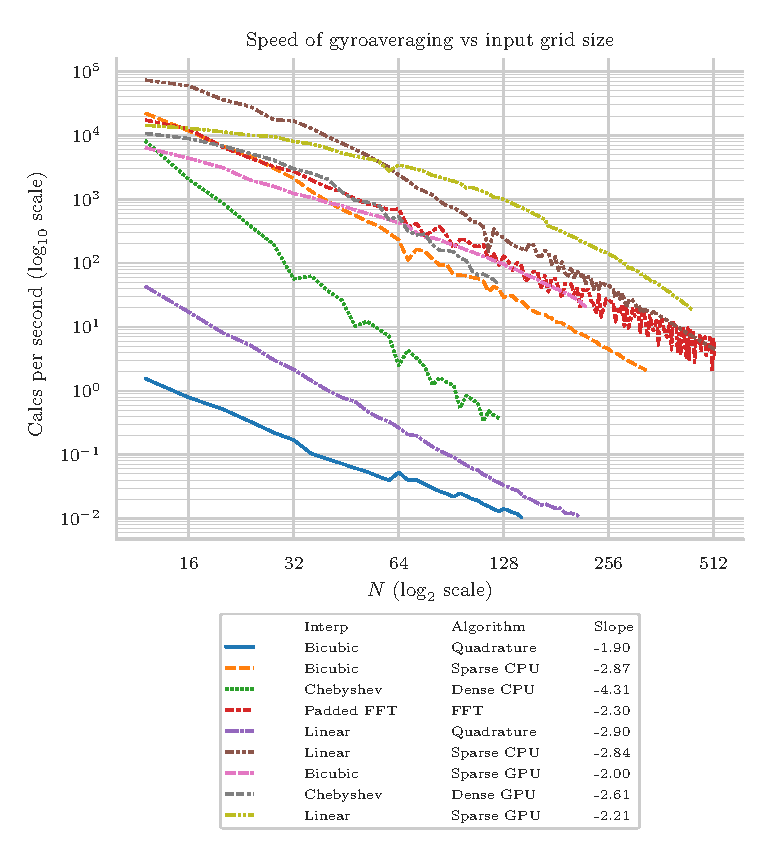
\includegraphics[scale=1]{SpeedVsN.eps}	
 	\caption{Calculation speed as grid size grows.  The slope is a linear regression coefficient for the displayed log-log plot.   Note that while the CPU-bound Chebyshev algorithm exhibits worse than quartic scaling, the GPU version scales with lower exponent (-2.61); this reflects the significance of the cost of CPU-GPU memory transfer which scales like $N^2$. }  	\end{figure}
	
	
	\begin{figure}[htbp!]
		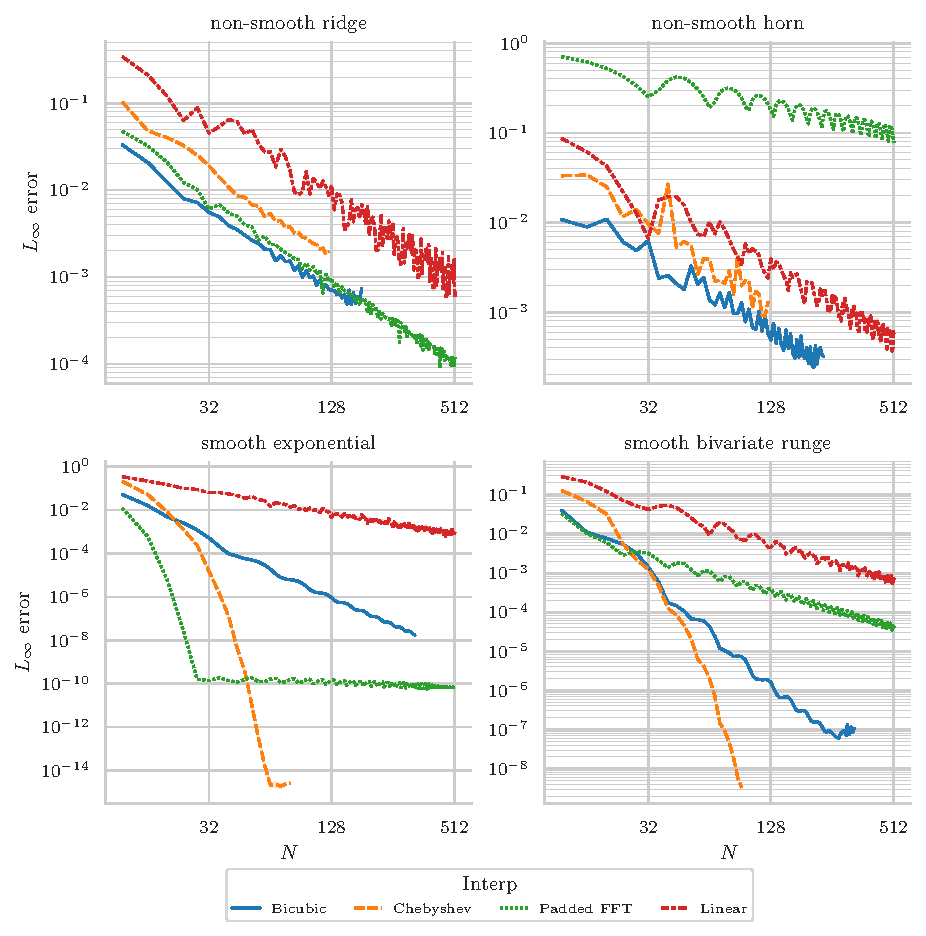
\includegraphics[scale=1]{ConvergenceAllNew.pdf}	
		\caption{Error vs grid size.  By construction, no one algorithm is a clear winner.  For smooth functions, we get spectral accuracy from the chebyshev interplation, and the Fourier method as well in the numerically periodic case.     }  	\end{figure}

	\begin{figure}[htbp!]
	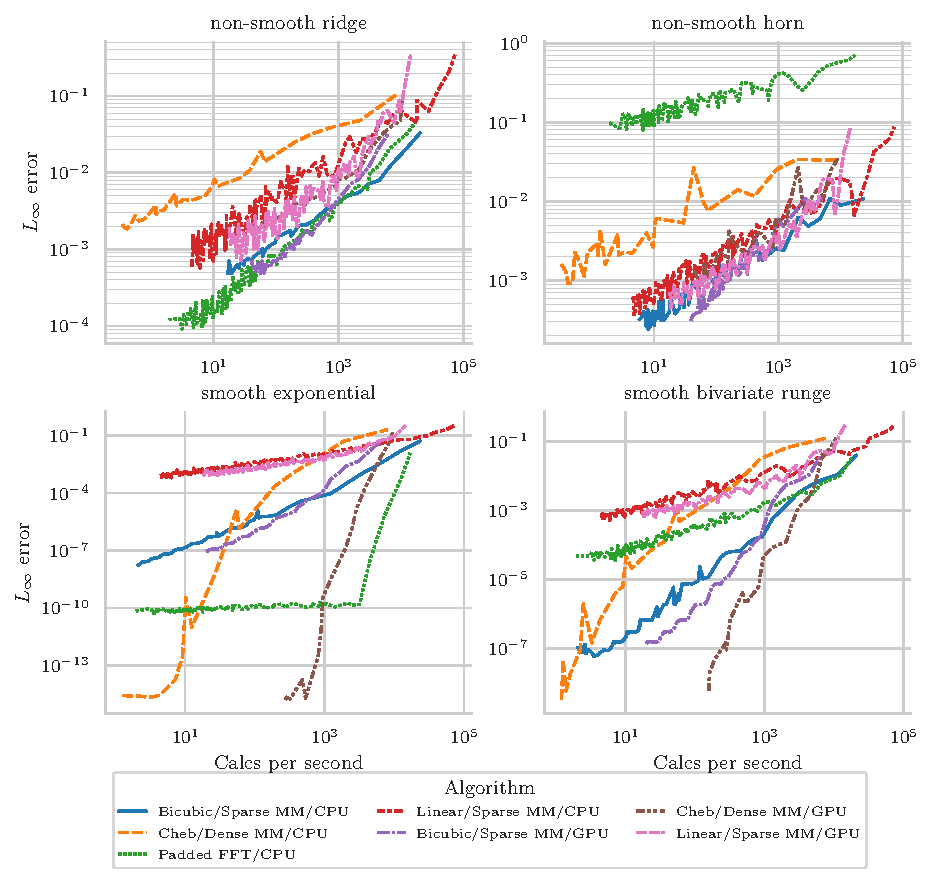
\includegraphics[scale=1]{OptimalAllNew.pdf}	
	\caption{The trade-off between accuracy and execution speed.     }  	\end{figure}


	
	
\end{enumerate}  






